% Compile with: xelatex helgarfri_cv_es.tex
% For exact website look, install Fira Code and use: \setmainfont{Fira Code}

\documentclass[11pt,a4paper]{article}

\usepackage[utf8]{inputenc}
\usepackage[T1]{fontenc}
\usepackage{fontspec}
\usepackage{geometry}
\usepackage{xcolor}
\usepackage{hyperref}
\usepackage{fontawesome5}
\usepackage{tcolorbox}
\usepackage{tikz}
\usepackage{enumitem}
\usepackage{ragged2e}
\usepackage{graphicx}
\usepackage{paracol}
\usepackage{eso-pic}

\geometry{a4paper, left=0pt, top=0pt, right=0.5in, bottom=0.5in}
\newlength{\sidebarwidth}
\AddToShipoutPictureBG{\AtPageLowerLeft{\textcolor{sidebar}{\rule{\sidebarwidth}{\paperheight}}}}
\newlength{\photoheight}
\setlength{\photoheight}{236pt}
\AddToShipoutPictureBG*{\AtPageUpperLeft{\raisebox{-\photoheight}{\begin{tikzpicture}[x=1pt, y=1pt]
  \useasboundingbox (0,0) rectangle (\sidebarwidth, \photoheight);
  \path[clip] (0, \photoheight) -- (\sidebarwidth, \photoheight) -- (\sidebarwidth, 0) -- (0, 51) -- cycle;
  \node[anchor=south west, inner sep=0, outer sep=0] at (0,0) {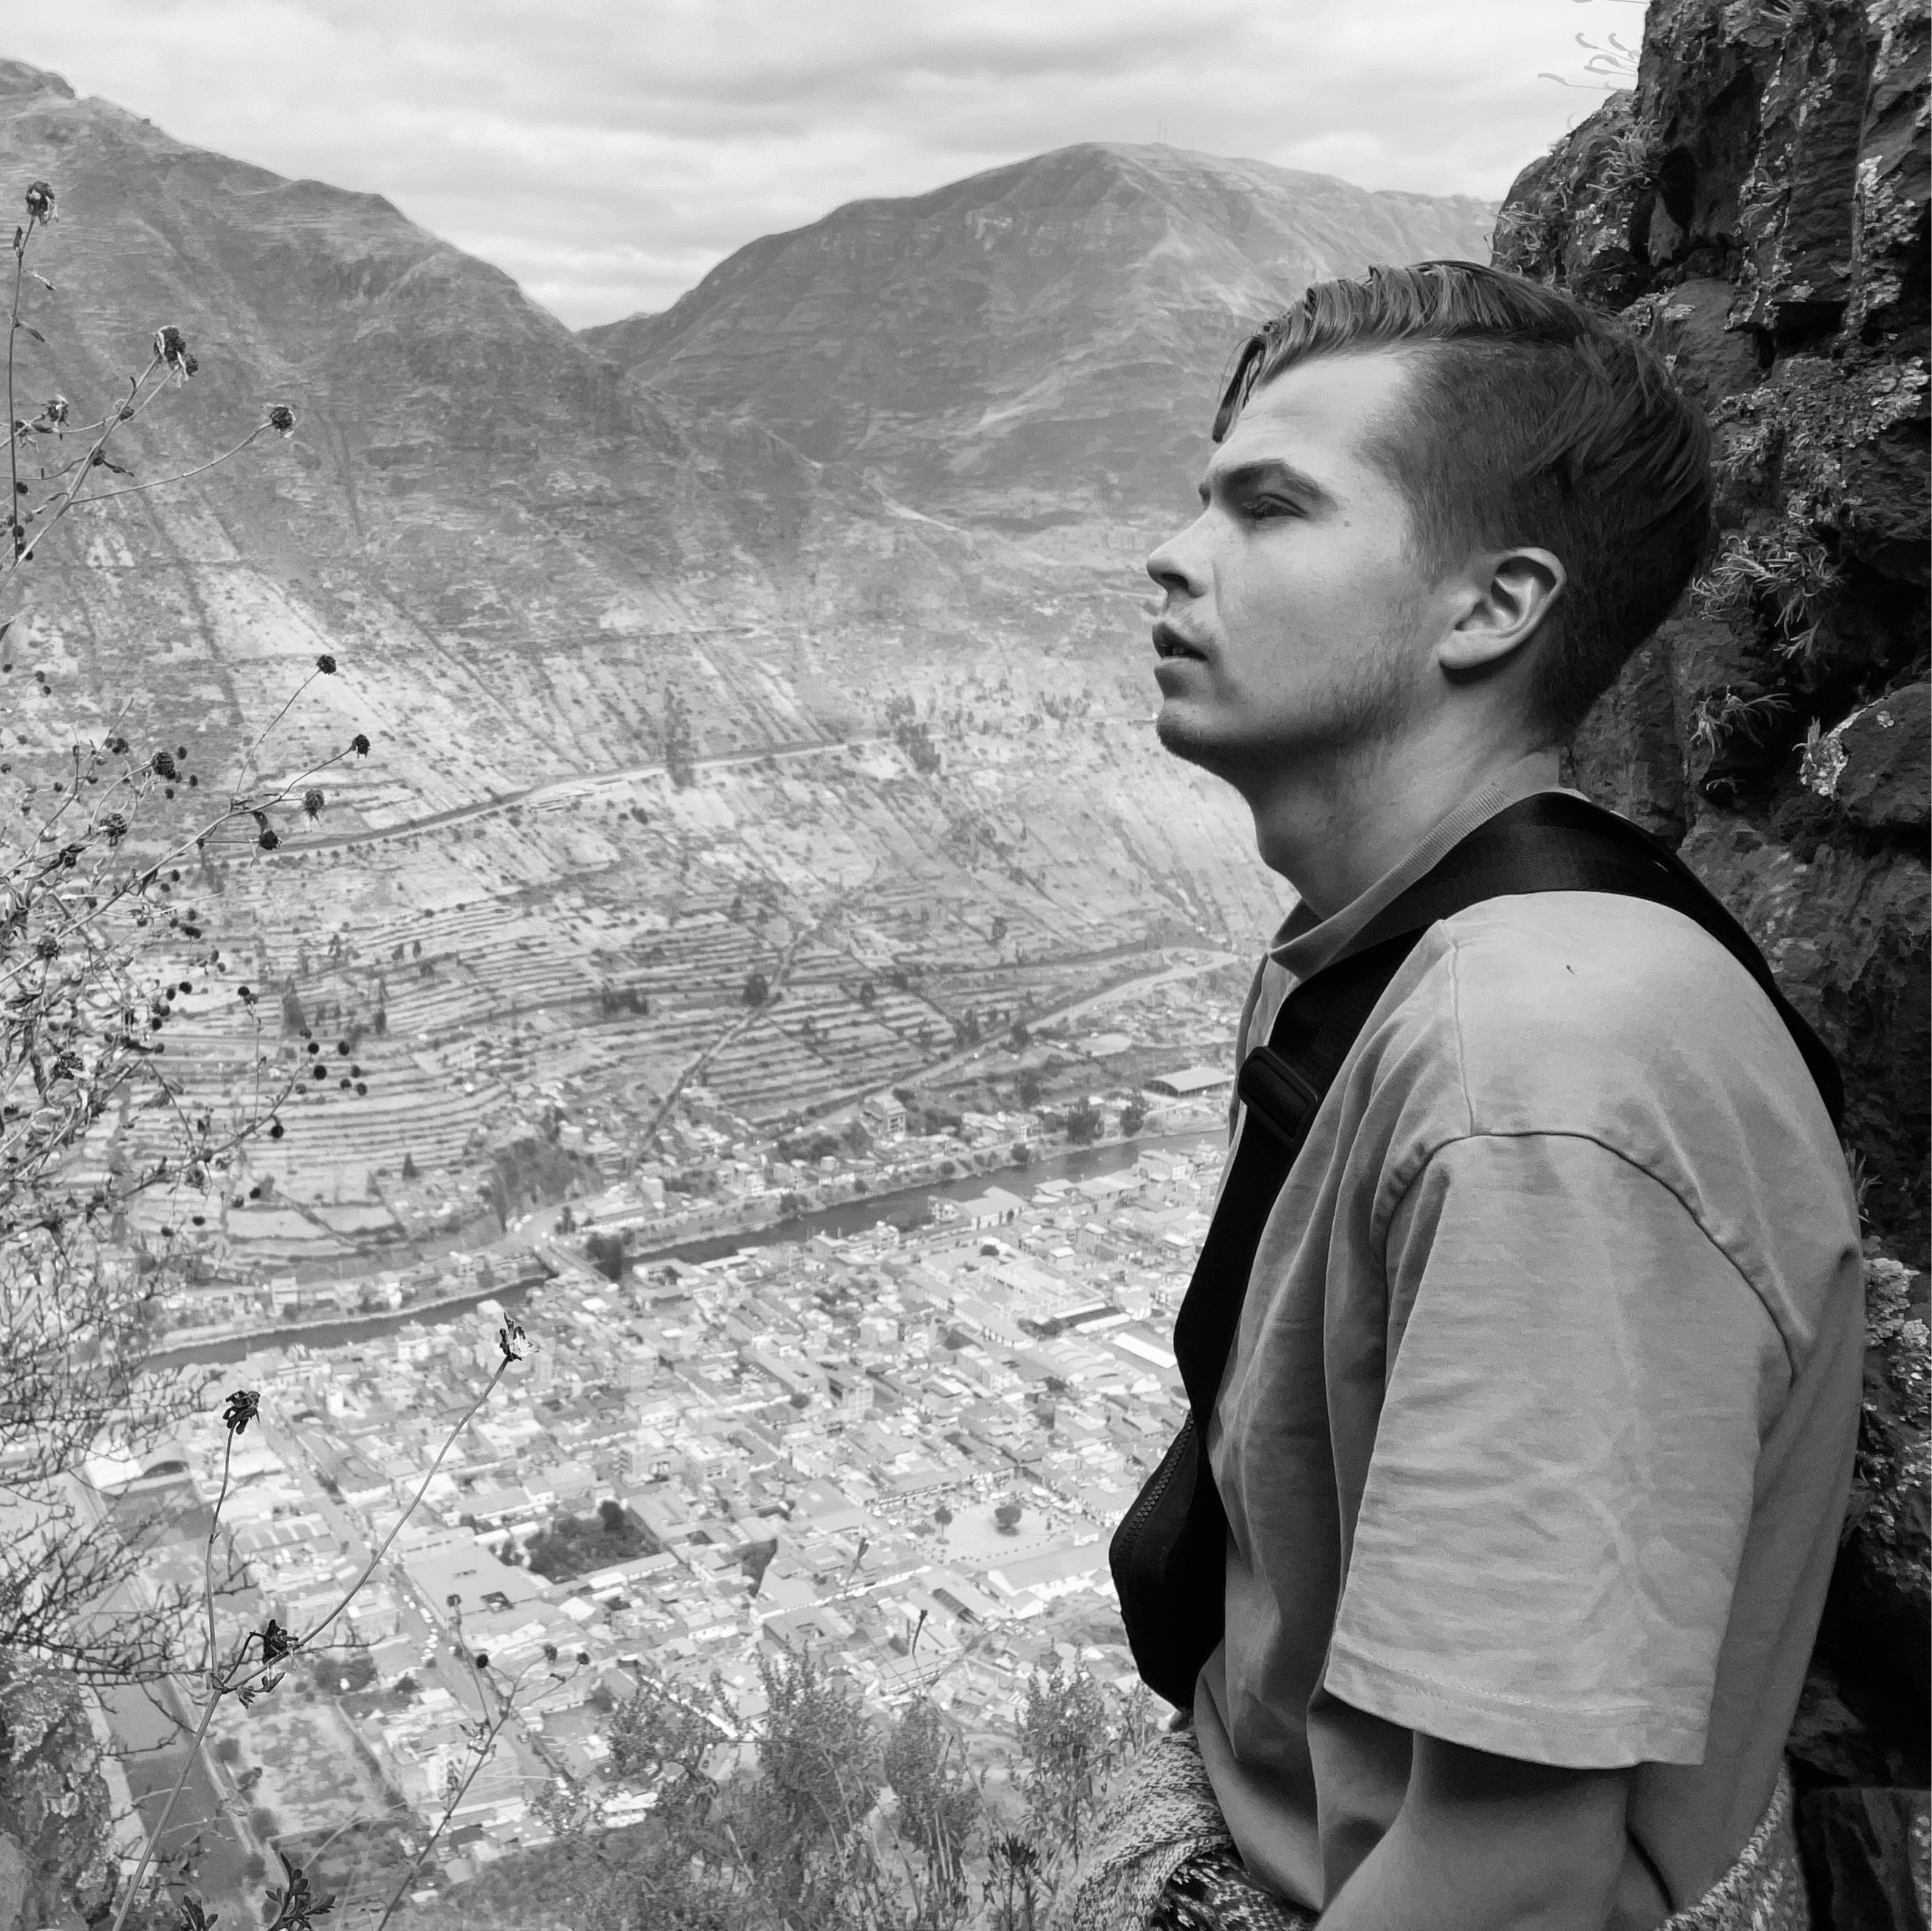
\includegraphics[width=\sidebarwidth, keepaspectratio=true]{helgarfri-cropped.jpg}};
\end{tikzpicture}}}}
\setmonofont{DejaVu Sans Mono}[Scale=0.92]
\renewcommand{\familydefault}{\ttdefault}

\pagestyle{empty}
\RaggedRight
\linespread{1.26}\selectfont

\definecolor{textcolor}{HTML}{1a1a1a}
\definecolor{boxbg}{HTML}{fafafa}
\definecolor{boxborder}{HTML}{e8e8e8}
\definecolor{linkcolor}{HTML}{1a1a1a}
\definecolor{sidebar}{HTML}{242424}
\definecolor{sidebartext}{HTML}{e8e8e8}
\definecolor{sidebarhead}{HTML}{cccccc}

\hypersetup{colorlinks=true, urlcolor=linkcolor, linkcolor=linkcolor}

\newcommand{\sidebarhead}[1]{%
  \textcolor{sidebarhead}{\textbf{\small #1}}\\[0.35em]%
}

\newcommand{\rightsection}[1]{%
  \vspace{1.5em}%
  \noindent\textcolor{textcolor}{\textbf{\large #1}}\\[0.4em]%
  \noindent\rule{0.25\textwidth}{0.35pt}\\[0.55em]%
}

\begin{document}
\setlength{\sidebarwidth}{0.41\textwidth}
\addtolength{\textheight}{22pt}

\vspace*{0pt}%
\noindent
\setcolumnwidth{0.41\textwidth, 0.56\textwidth}
\setlength{\columnsep}{0pt}
\begin{paracol}{2}

  \parbox[t]{\linewidth}{%
    \parindent=0pt
    \color{sidebartext}\small\raggedright
    \setlength{\baselineskip}{1.12\baselineskip}%
  \rule{0pt}{\photoheight}%
  \vspace{0.22em}%
  \leftskip=30pt \rightskip=30pt

  \sidebarhead{presentación breve}
  soy desarrollador y futuro informático, con enfoque en desarrollo web.
  tengo experiencia construyendo un stack web completo desde cero con express.js y postgresql.
  me gusta resolver problemas y quiero trabajar en proyectos exigentes de ingeniería de datos, desarrollo de software o análisis.
  \vspace{1.2em}

  \sidebarhead{contacto}
  \faPhone\ +354 837 8222\\[0.25em]
  \faEnvelope\ \href{mailto:helgi@helgarfri.is}{\textcolor{sidebartext}{helgi@helgarfri.is}}\\[0.25em]
  \faGithub\ \href{https://github.com/helgarfri}{\textcolor{sidebartext}{helgarfri}}\\[0.25em]
  \faGlobe\ \href{https://helgarfri.is}{\textcolor{sidebartext}{helgarfri.is}}\\[0.25em]
  \faMapMarker*\ ólafsgeisli 89, 113 reikiavik
  \vspace{1.2em}

  \sidebarhead{competencias}
  \begin{itemize}[left=3.2em, nosep, itemsep=0.22em]
    \item javascript / typescript
    \item node.js / express
    \item postgresql
    \item git / github
    \item react.js / next.js, html / css
  \end{itemize}
  \vspace{0.85em}

  \sidebarhead{idiomas}
  \begin{itemize}[left=3.2em, nosep, itemsep=0.28em]
    \item islandés — nativo
    \item inglés — fluido
    \item español — intermedio
  \end{itemize}
  }%

\switchcolumn

\leftskip=0.2in \rightskip=0.05in
\sloppy
\vspace{4.5em}
\textcolor{textcolor}{%
  {\Huge\textbf{helgi freyr davíðsson}}\\[0.4em]
  \normalsize desarrollador / estudiante de informática
  \vspace{1.2em}
}

\rightsection{experiencia laboral}
\textbf{profesor de programación} \hfill {\small 2026 - actualidad}\\[0.15em]
\small tjarnarskóli\\[0.25em]
\small enseñanza de programación web (HTML, CSS, JavaScript) en educación primaria; diseño de tareas y acompañamiento en fundamentos web.
\vspace{0.6em}

\textbf{administrador de sistemas} \hfill {\small 2025 - actualidad}\\[0.15em]
\small universidad de islandia, asociación de estudiantes\\[0.25em]
\small desarrollo y mantenimiento de backend y frontend, gestión de plataformas digitales, fiabilidad y colaboración con juntas.
\vspace{0.6em}

\textbf{responsable de líneas / reposición} \hfill {\small 2023 - 2025}\\[0.15em]
\small ölgerðin egill skallagrímsson\\[0.25em]
\small reposición de grifos, pedidos mediante el sistema de inventario y abastecimiento continuo de bebidas.
\vspace{1.25em}

\textbf{responsable de recepción} \hfill {\small 2019 - 2023}\\[0.15em]
\small club de golf de mosfellsbær\\[0.25em]
\small atención a socios, venta y relación con visitantes, reservas y gestión de membresías.

\rightsection{proyectos}
\textbf{map in color} \href{https://mapincolor.com}{(mapincolor.com)} \hfill {\small 2023 - actualidad}\\[0.25em]
\small
plataforma para crear, descubrir y compartir mapas basados en datos: mapas numéricos o categóricos, importación CSV/TSV/Excel, descubrimiento y uso compartido. se puede probar sin registrarse.

\rightsection{formación}
\textbf{grado en informática} \hfill {\small 2023 - presente}\\[0.15em]
\small universidad de islandia (ECTS: 136,5/180, previsto 2026)\\[0.6em]

\textbf{intercambio en informática} \hfill {\small 2025}\\[0.15em]
\small universidad complutense de madrid\\[0.6em]

\textbf{bachillerato} \hfill {\small 2018 - 2022}\\[0.15em]
\small framhaldsskólinn í mosfellsbæ

\end{paracol}

\end{document}
